

有几种方法可以将依赖项作为源获取到项目中。一种相对直接(但危险)的方法是,将代码手动下载或克隆到项目内的子文件夹,然后使用\texttt{add\_subdirectory}添加这个文件夹。虽然这样做很有效,而且速度很快,但很快就会变得乏味且难以维护。所以,这应该尽可能实现自动化。

\begin{tcolorbox}[colback=webgreen!5!white,colframe=webgreen!75!black,title=Note]
下载并将第三方软件的副本集成到产品中的做法,称为供应商方式。优点是常常使构建软件变得容易,但在打包库方面产生了问题。通过使用包管理器或在系统上的某个位置安装第三方软件,可以避免使用供应商方式。
\end{tcolorbox}

\subsubsubsection{5.5.1\hspace{0.2cm}下载依赖项作为源代码}

获取外部内容的基础模块是\texttt{ExternalProject}模块和更复杂的\texttt{FetchContent}模块,后者使用了\texttt{ExternalProject}。虽然\texttt{ExternalProject}提供了更多的灵活性,但\texttt{FetchContent}使用起来更方便,特别是下载的项目也可以使用CMake构建。它们都将项目作为源文件下载,并可用于构建当前项目。

\hspace*{\fill} \\ %插入空行
\noindent
\textbf{使用FetchContent}

对于构建的外部项目,使用\texttt{FetchContent}模块是添加源依赖项的一种方法。对于二进制依赖,使用\texttt{find\_package}和Find<PackageName>.cmake式的方式仍是首选。\texttt{ExternalProject}和\texttt{FetchContent}之间的主要区别是,\texttt{FetchContent}可以在配置时下载和配置外部项目,而\texttt{ExternalProject}需要在构建时中完成所有工作。这样做的缺点是,源及其配置在配置时不可用。

没使用\texttt{FetchContent}之前,需要使用Git子模块手动下载依赖项,然后使用\texttt{add\_subdirectory}添加源。在某些情况下这是可行的,但维护起来则会很麻烦。

\texttt{FetchContent}提供了一系列函数来拉取源依赖项,主要是\texttt{FetchContent\_Declare},它定义了下载和构建\texttt{FetchContent\_MakeAvailable}的参数,\texttt{FetchContent\_MakeAvailable}填充依赖项的目标,并使它们可用于构建。下面的例子中,bertrand库是通过Git将代码从GitHub上拉下来的:

\begin{lstlisting}[style=styleCMake]
include(FetchContent)
FetchContent_Declare(
	bertrand
	GIT_REPOSITORY https://github.com/bernedom/bertrand.git
	GIT_TAG 0.0.17)

FetchContent_MakeAvailable(bertrand)

add_executable(fetch_content_example)
target_link_libraries(
	fetch_content_example
	PRIVATE bertrand::bertrand
)
\end{lstlisting}

3.14版本之后,可以使用\texttt{FetchContent\_MakeAvailable},建议通过使用\texttt{FetchContent\_Populate}手动填充项目,因为它的简单性使代码库非常可维护。和\texttt{ExternalProject}一样,\texttt{FetchContent}也可以从HTTP(S)、Git、SVN、Mercurial和CVS下载,相应的实践(例如为下载的内容指定MD5哈希值或使用Git哈希值)也适用。

\texttt{FetchContent\_MakeAvailable}是使基于CMake的外部项目可用的推荐方法,但若想对外部项目有更多的控制,也可以手动填充项目。下面的示例与前面的示例相同,但更详细:

\begin{lstlisting}[style=styleCMake]
FetchContent_Declare(
	bertrand
	GIT_REPOSITORY https://github.com/bernedom/bertrand.git
	GIT_TAG 0.0.17)
	
if(NOT bertrand_POPULATED)
	FetchContent_Populate(bertrand)
	add_subdirectory(${bertrand_SOURCE_DIR} ${bertrand_BINARY_DIR})
endif()
\end{lstlisting}

\texttt{FetchContent\_Populate}需要指定的附加选项,可以更细粒度地控制构建。签名如下:

\begin{lstlisting}[style=styleCMake]
FetchContent_Populate( <name>
	[QUIET]
	[SUBBUILD_DIR <subBuildDir>]
	[SOURCE_DIR <srcDir>]
	[BINARY_DIR <binDir>]
	...
)
\end{lstlisting}

来看看\texttt{FetchContent\_Populate}的选项:

\begin{itemize}
\item 
QUIET: 若成功,可以指定此值来抑制屏幕输出。若失败,即使指定了允许调试的选项,也会显示输出。

\item
SUBBUILD\_DIR: 这指定了外部项目的位置。默认值是\$\{CMAKE\_CURRENT\_BINARY\_DIR\}/ <name>-subbuild。通常,这个选项应该保持不变。

\item
SOURCE\_DIR和BINARY\_DIR: 这更改了外部项目的源目录和构建目录的位置。对于SOURCE\_DIR,默认设置为\$\{CMAKE\_CURRENT\_BINARY\_DIR\}/<lcname>-src;对于BINARY\_DIR,默认设置为\$\{CMAKE\_CURRENT\_BINARY\_DIR\}/<lcname>-build。

\item
添加的附加参数将传递到底层的\texttt{ExternalProject\_Add}。然而,\texttt{FetchContent}禁止编辑不同步骤的命令,因此试图修改\texttt{CONFIGURE\_COMMAND}、\texttt{BUILD\_COMMAND}、\texttt{INSTALL\_COMMAND}和\texttt{TEST\_COMMAND}的操作,将导致\texttt{FetchContent\_Populate}的失败,并显示相应的错误信息。
\end{itemize}

\begin{tcolorbox}[colback=webgreen!5!white,colframe=webgreen!75!black,title=Note]
若发现自己处于需要将选项传递给底层\texttt{ExternalProject\_Add}的情况下,可以考虑直接使用\texttt{ExternalProject}。
\end{tcolorbox}

关于源和构建目录的信息,以及项目是否填充,可以通过读取<name>\_SOURCE\_DIR、<name>\_BINARY\_DIR和<name>\_POPULATED变量或使用\texttt{FetchContent\_GetProperties}来检索。注意<name>或是全大写,或是全小写。尽管大小写不同,这是为了让CMake识别不同的包。
 
\texttt{FetchContent}的另一个优势是,可以处理外部项目的公共依赖,并避免多次下载和构建。第一次在\texttt{FetchContent}上定义依赖时会缓存,之后的定义都会忽略。这样做可让父项目可以改写子项目的依赖关系。

假设有一个名为MyProject的顶层项目,它获取两个外部项目,project\_A和project\_B,每个项目都依赖于名为AwesomeLib的外部项目,但依赖于不同的版本。通常,我们不想下载和使用两个版本的AwesomeLib,只想使用一个版本以避免冲突。下图显示了目前依赖关系的样子:

\begin{center}
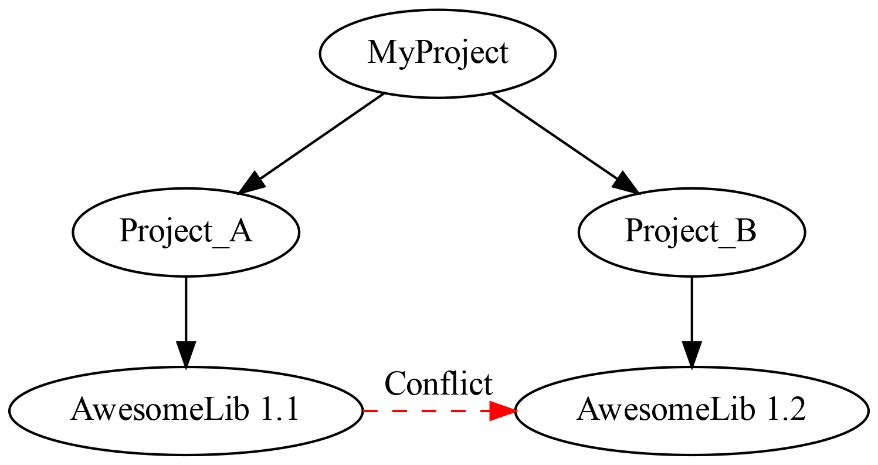
\includegraphics[width=0.6\textwidth]{content/2/chapter5/images/1.jpg}\\
图5.1  Project\_A和Project\_B依赖于不同版本的AwesomeLib
\end{center}

为了解决这个问题,可以通过在顶层的CMakeLists.txt文件中使用\texttt{FetchContent\_Declare}对AwesomeLib进行调用,来指定要提取哪个版本的AwesomeLib。这里,CMakeLists.txt文件中声明的顺序并不重要,重要的是声明级别。因为Project\_A和Project\_B都使用了AwesomeLib的源码,所以顶层项目不需要使用\texttt{FetchContent\_MakeAvailable}或\texttt{FetchContent\_Populate}:

\begin{lstlisting}[style=styleCMake]
include(FetchContent)
FetchContent_Declare(Project_A GIT_REPOSITORY ... GIT_TAG ...)
FetchContent_Declare(Project_B GIT_REPOSITORY ... GIT_TAG ...)

# Force AwesomeLib dependency to a certain version
FetchContent_Declare(AwesomeLib
	GIT_REPOSITORY … GIT_TAG 1.2 )
FetchContent_MakeAvailable(Project_A)
FetchContent_MakeAvailable(Project_B)
\end{lstlisting}

这将使所有项目都使用AwesomeLib的1.2版本。当然,只有当Project\_A和Project\_B需要的版本之间的接口是兼容的情况下,才有以下依赖:

\begin{center}
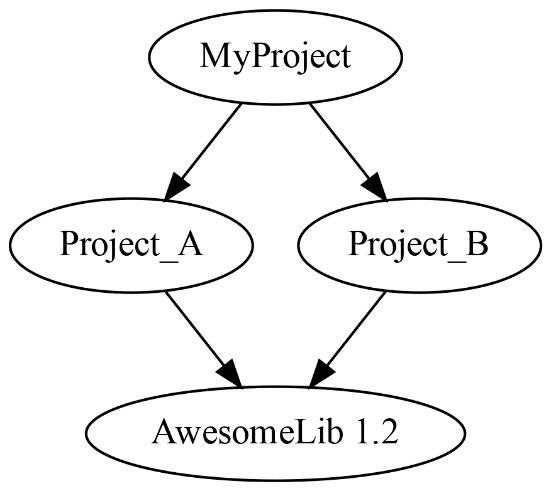
\includegraphics[width=0.4\textwidth]{content/2/chapter5/images/2.jpg}\\
图5.2  MyProject声明了AwesomeLib版本后的依赖关系图
\end{center}

添加依赖项作为源有优点,也有缺点,这会增加了配置和构建时间。第9章中,我们将使用分布式库处理超级构建,并提供关于处理源依赖关系的更多信息。

本章的开头,讨论了\texttt{find\_package},其可以用来包含二进制依赖项,但是没有讨论如何使用CMake方便地下载本地二进制依赖项。虽然\texttt{FetchContent}和\texttt{ExternalProject}可以用,但这不是其目的。相反,使用专门的包管理器会更合适,如Conan和vcpkg。

\hspace*{\fill} \\ %插入空行
\noindent
\textbf{使用ExternalProject}

\texttt{ExternalProject}模块用于下载和构建未集成到主项目中的外部项目。构建外部项目时,构建完全隔离,不会自动接管与架构或平台相关的设置。这种隔离可以避免在命名目标或组件时发生冲突。外部项目创建主目标和几个包含以下独立构建步骤的子目标:

\begin{enumerate}
\item 
下载: \texttt{ExternalProject}可以通过几种方式下载内容,例如HTTPS下载,或者通过访问版本控制系统,如Git、Subversion、Mercurial和CVS。若内容打包,下载后将进行解包操作。

\item 
更新和打补丁: 若从Server Configuration Monitor (SCM)提取内容,则可以对下载的源代码进行打补丁或更新到最新版本。

\item 
配置: 若下载的源代码使用CMake,则在其上执行配置步骤。对于非CMake项目,可以提供执行配置的自定义命令。

\item 
构建: 默认情况下,用于构建依赖项的构建工具与主项目中使用的构建工具相同,但若不这样做,可以提供自定义命令。若提供了自定义构建命令,则由用户来确保传递必要的编译器标志。

\item 
安装: 隔离构建可以在本地安装,通常安装在主项目的构建树中的某个位置。

\item 
测试: 若外部内容附带测试,则主项目可以选择性运行。通常,不运行测试。
\end{enumerate}

包括下载在内的所有步骤都在构建时运行,根据外部项目的不同,这增加了构建的耗时。CMake缓存下载和构建,开销主要是第一次运行时的耗时,除非外部项目进行了更改。可以向外部构建添加更多步骤,但对于大多数项目,默认的步骤已经足够了。这些步骤可以自定义,也可以省略。

以下示例中,bertrand库通过HTTPS下载,并安装在当前构建目录中:

\begin{lstlisting}[style=styleCMake]
include(ExternalProject)
ExternalProject_Add(
	bertrand
	URL https://github.com/bernedom/bertrand/archive
	/refs/tags/0.0.17.tar.gz
	URL_HASH MD5=354141c50b8707f2574b69f30cef0238
	INSTALL_DIR ${CMAKE_CURRENT_BINARY_DIR}/bertrand_install
	CMAKE_CACHE_ARGS -DBERTRAND_BUILD_TESTING:BOOL=OFF
	-DCMAKE_INSTALL_PREFIX:PATH=<INSTALL_DIR>
)
\end{lstlisting} 

\texttt{ExternalProject}模块在默认情况下不可用,必须通过\texttt{include(ExternalProject)}将其包含在第一行中。由于外部库安装在本地构建目录中,因此指定了INSTALL\_DIR。由于bertrand本身是一个CMake项目,可以通过CMAKE\_INSTALL\_PREFIX来构建项目,安装目录为<INSTALL\_DIR>(一个占位符),指向INSTALL\_DIR选项。\texttt{ExternalProject}了解各种目录的占位符,例如<SOURCE\_DIR>、<BINARY\_DIR>和<DOWNLOAD\_DIR>。完整的列表,请参考模块文档\url{https://cmake.org/cmake/help/latest/module/ExternalProject.html}。

\begin{tcolorbox}[colback=blue!5!white,colframe=blue!75!black,title=下载验证]
强烈建议将为下载URL添加哈希码,因为若工件的内容发生更改,这会将让您知晓。
\end{tcolorbox}

为此,依赖bertrand的目标都必须在外部依赖之后构建。由于bertrand是一个纯头文件的库,所以想要将include路径添加到目标。在CMake中目标使用外部项目:

\begin{lstlisting}[style=styleCMake]
ExternalProject_Get_Property(bertrand INSTALL_DIR)
set(BERTRAND_DOWNLOADED_INSTALL_DIR "${INSTALL_DIR}")

# Create a target to build an executable
add_executable(external_project_example)

# make the executable to be built depend on the external project
# to force downloading first
add_dependencies(external_project_example bertrand)

# make the header file for bertrand available
target_include_directories(external_project_example PRIVATE
${BERTRAND_DOWNLOADED_INSTALL_DIR}/include)
\end{lstlisting}

第一行中,使用\texttt{ExternalProject\_Get\_Property}检索安装目录,并将其存储在INSTALL\_DIR中。但变量名总是与属性相同,因此建议在检索后立即将其存储在具有惟一名称的变量中。

接下来,创建目标并依赖于\texttt{ExternalProject\_Add}的目标。这对于执行构建的正确顺序很有必要。

最后,使用\texttt{target\_include\_directories}将安装路径添加到目标。此外,若外部项目不是由CMake构建的,可以导入由外部库提供的CMake目标。

通过相应的选项从源代码管理系统下载。对于Git,通常像这样:

\begin{lstlisting}[style=styleCMake]
ExternalProject_Add(MyProject GIT_REPOSITORY
	https://github.com/PacktPublishing/SomeRandomProject.git
		GIT_TAG 56cc1aaf50918f208e2ff2ef5e8ec0111097fb8d )
\end{lstlisting}

GIT\_TAG可以是任何有效提交版本号,包括标记名和长、短哈希码。若省略GIT\_TAG,则会下载默认分支(通常称为main或master)的最新版本,建议下载指定版本。因为标签和分支可以修改(尽管在实践中很少这样做),所以最健壮的方法是定义一个提交哈希码。SVN与从Git类似,更多细节请参考官方文档。

\hspace*{\fill} \\ %插入空行
\noindent
\textbf{处理非CMake项目和交叉编译}

\texttt{ExternalProject}的一个常见用例是构建依赖关系,有时需要使用CMake之外的工具进行处理,比如:autotools或automake。这时,需要指定如下的配置和构建命令:

\begin{lstlisting}[style=styleCMake]
find_program(MAKE_EXECUTABLE NAMES nmake gmake make)
ExternalProject_Add(MyAutotoolsProject
	URL someUrl
	INSTALL_DIR ${CMAKE_CURRENT_BINARY_DIR}/myProject_install
	CONFIGURE_COMMAND <SOURCE_DIR>/configure --prefix=<INSTALL_DIR>
	BUILD_COMMAND ${MAKE_EXECUTABLE}
)
\end{lstlisting}

第一个\texttt{find\_program}用于查询make的版本,并将其存储在MAKE\_EXECUTABLE变量中。外部项目的一个常见问题是,必须控制依赖项的安装位置。大多数项目都希望安装到默认的系统位置,这通常需要Root特权,可能会污染系统,可以将必要的选项传递给配置或构建步骤。另一种处理方法是将INSTALL\_COMMAND替换为一个空字符串来完全避免安装过程:

\begin{lstlisting}[style=styleCMake]
ExternalProject_Add(MyAutotoolsProject
	URL someUrl
	CONFIGURE_COMMAND <SOURCE_DIR>/configure
	BUILD_COMMAND ${MAKE_EXECUTABLE}
	INSTALL_COMMAND ""
)
\end{lstlisting}

使用此类的非CMake项目的问题是,它们没有为直接使用依赖定义必要的目标,为了在另一个目标中使用外部构建的库,通常必须将完整的库名称添加到\texttt{target\_link\_libraries}中,这样做的缺点是必须手动维护不同平台的文件的不同名称和位置。\texttt{find\_library}或\texttt{find\_file}发生在配置时,所以对于\texttt{ExternalProject}没有用,\texttt{ExternalProject}只在构建时才创建必要的文件。

另一个常见的用例是\texttt{ExternalProject}为不同的目标平台构建现有源目录的内容。本例中,直接省略了处理下载的参数。若外部项目使用CMake进行构建,则可以将工具链文件作为CMake选项传递给外部项目。这里有常见问题是,\texttt{ExternalProject}不会识别外部项目源的更改,因此CMake可能不会重新构建它们。因此,应该传递BUILD\_ALWAYS选项,其缺点是使构建时间变长:

\begin{lstlisting}[style=styleCMake]
ExternalProject_Add(ProjectForADifferentPlatform
SOURCE_DIR 
	${CMAKE_CURRENT_LIST_DIR}/ProjectForADifferentPlatform
INSTALL_DIR ${CMAKE_CURRENT_BINARY_DIR}/
	ProjectForADifferentPlatform-install
CMAKE_ARGS
	-D CMAKE_TOOLCHAIN_FILE=${CMAKE_CURRENT_LIST_DIR}/fwtoolchain.cmake
	-D CMAKE_BUILD_TYPE=Release
	-D CMAKE_INSTALL_PREFIX=<INSTALL_DIR>
BUILD_ALWAYS YES
)
\end{lstlisting}

\hspace*{\fill} \\ %插入空行
\noindent
\textbf{管理ExternalProject中的步骤}

如上一节所述,可以进一步配置\texttt{ExternalProject}的步骤,并以更细粒度的方式使用。通过传递STEP\_TARGETS选项或使用\texttt{ExternalProject\_Add\_StepsTargets},告诉\texttt{ExternalProject}为每个步骤创建常规目标。以下调用将外部项目的配置步骤和构建步骤形成目标:

\begin{lstlisting}[style=styleCMake]
ExternalProject_Add(MyProject
	# various options
	STEP_TARGETS configure build
)
ExternalProject_Add_StepTargets(MyProject configure build)
\end{lstlisting}

目标以<mainName>-step命名。前面的示例中,将创建另外两个目标,MyProject-configure和MyProject-build。创建步骤目标有两个主要用途:可以创建按照下载、配置、构建、安装或测试顺序排序的自定义步骤,或者可以使步骤依赖于其他目标。这些目标可以是普通的目标,通过\texttt{add\_executable}、\texttt{add\_library}或\texttt{add\_custom\_target}创建,也可以添加入其他可执行文件的目标中。常见的情况是外部项目相互依赖,因此一个项目的配置步骤必须依赖另一个项目。下一个例子中,项目B的配置步骤将取决于项目A的完成情况:
 
\begin{lstlisting}[style=styleCMake]
ExternalProject_Add(ProjectA
	... # various options
		STEP_TARGETS install
)
ExternalProject_Add(ProjectB
... # various options
)
ExternalProject_Add_StepDependencies(ProjectB configure ProjectA)
\end{lstlisting}

最后,还可以创建插入到外部项目中的自定义步骤。添加步骤可以通过\texttt{ExternalProject\_Add\_Step}指令完成。自定义步骤的名称不能与预定义步骤相同(例如创建文件夹、下载、更新、补丁、配置、构建、安装或测试)。下面的示例将创建一个步骤,构建后将外部项目的许可信息添加到特定的tar文件中:

\begin{lstlisting}[style=styleCMake]
ExternalProject_Add_Step(bertrand_downloaded copy_license
	COMMAND ${CMAKE_COMMAND} -E tar "cvzf"
		${CMAKE_CURRENT_BINARY_DIR}/licenses.tar.gz <SOURCE_DIR>/LICENSE
	DEPENDEES build
)
\end{lstlisting}

总之,\texttt{ExternalProject}是一个非常强大的工具,但管理起来可能会很复杂,正是这种灵活性也使得\texttt{ExternalProject}难以使用。虽然可以隔离构建,但它需要项目维护者手动将来自外部项目内部工作的信息公开给CMake。更具有讽刺意味的是,这正是CMake最初所不愿看到的情况。











